\documentclass[12pt]{article}

\usepackage{graphicx}
\usepackage{epstopdf}


\usepackage[spanish]{babel} % silabea palabras castellanas <- Puedo poner comentarios para explicar de que va este comando en la misma línea
\selectlanguage{spanish} 

%Encoding
\usepackage[utf8]{inputenc} % Acepta caracteres en castellano
\usepackage[T1]{fontenc} % Encoding de salida al pdf

%Triunfó el mal
\usepackage[normalem]{ulem}
\useunder{\uline}{\ul}{}
\providecommand{\e}[1]{\ensuremath{\times 10^{#1}}}
\usepackage{quotmark} %Uso consistente con la RAE de comillas
\usepackage{listings} % Comandos de la terminal

\usepackage{textcomp}
\usepackage{gensymb}


%Hipertexto
\usepackage[colorlinks=true,urlcolor=blue,linkcolor=blue]{hyperref} % navega por el doc: hipertexto y links

%Aquello de las urls
\usepackage{url} 

%simbolos matemáticos
\usepackage{amsmath}
\usepackage{amsfonts}
\usepackage{amssymb}
\usepackage{physics} %Best pack

% permite insertar gráficos, imágenes y figuras, en pdf o en eps
\usepackage{graphicx}
\usepackage{epstopdf}
\usepackage{multirow}
\usepackage{float}
\usepackage[export]{adjustbox}
% geometría del documento, encabezados y pies de páginas, márgenes
\usepackage{geometry}
\usepackage{comment}

%\usepackage[english]{babel}
%\usepackage[latin5]{inputenc}
% \usepackage{hyperref}
%\newdate{date}{10}{05}{2013}
%\date{\displaydate{date}}
\begin{document}




\title{Cúmulos Abiertos \\ Taller 3 Fotometría de Apertura IRAF}

\author{
\textbf{Javier Alejandro Acevedo Barroso\thanks{e-mail: \texttt{ja.acevedo12@uniandes.edu.co}}}\\
\textit{Universidad de los Andes, Bogotá, Colombia}\\
 }% Hasta aquí llega el bloque "author" (son dos autores por informe, orden alfabético)

\date{\today}
%\date{Versión $\alpha \beta$ fecha del documento}
\maketitle %Genera el título del documento


\normalsize
\newpage


\section{Función Inicial de Masa}
La función inicial de masa es la función que relaciona la masa al momento de entrar a la secuencia principal, con el número de estrellas en una población entrando a la secuencia principal con esa masa. Es decir, en una población estelar recien nacida de estrellas, la función inicial de masa correspondería completamente con el histograma de las masas. La importancia de la función inicial de masa radica en que la masa con la que una estrella entra a su secuencia principal es la variable más importante para determinar su evolución.



\section{Fotometría de apertura}
El objetivo de este ejercicio es realizar el procesamiento de fotometría de apertura para las imágenes del tutorial de IRAF. Esto corresponde a calcular una magnitud instrumental para los objetos del campo estelar. Por ser la primera vez que se realiza tal análisis, se realizará paso a paso y para un número límitado de estrellas. En futuros ejercicios se realizará el análisis para todo el campo, usando algoritmos implementados en IRAF para localizar los objetos.

Las imágenes se tomaron con instrumentos CCD y por lo tanto se realizaron las respectivas correcciones de FLAT, OVERSCAN y BIAS. El ejercicio asume que las imágenes ya están corregidas.





\subsection{Primer Camino}
Para realizar el proceso paso a paso, se debe empiezar definiendo la región del overscan que se utilizará en la corrección. Usualmente, a las imágenes astronómicas se les añade una serie de columnas (y/o filas) que corresponden a la lectura del CCD con cero fotones recolectados, es decir, el nivel \tqt{cero} u \tqt{offset}\cite{handbookCCD}. En el caso del ejercicio, se toma la imagen \tqt{92006.fits} y manualmente se busca su región de \tqt{overscan} . Esta región corresponde a las columnas 320 hasta el final de la imagen en 352. Adicionalmente, hay un gran pico de conteos en la columna 319, justo antes de empezar la región del \tqt{overscan} . Esto se puede observar en la siguiente imagen. \\

%\begin{figure}[H]
%  \centering
%   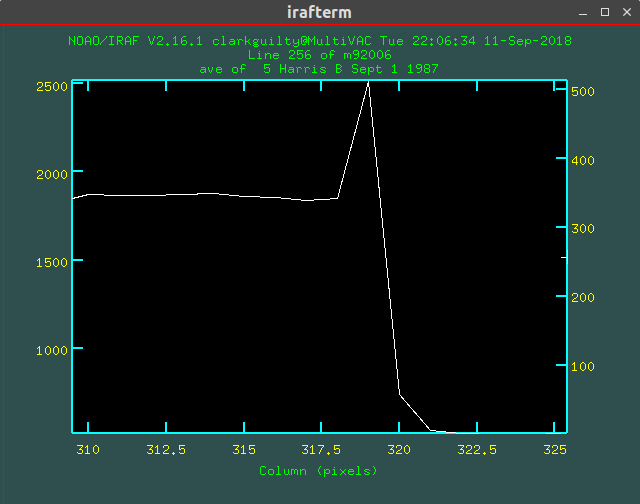
\includegraphics[scale= 0.5]{im01.png}
%  \caption{}
%  \label{im01}
%\end{figure}



Una vez identificado el overscan, se procede a definir los límites de la imagen real, es decir, la imagen sin el \tqt{overscan}  y el pico de conteos que los separa. Tras inspeccionar la imagen, se decidió que las columnas a promediar para el \tqt{offset} son de la 325 hasta la 350, esto con el fin de cubrir la mayor cantidad de columnas posibles sin incluir el pico. Para las filas se seleccionó desde la 4 hasta la 508, en este caso simplemente se dejó 4 pixeles de tolerancia con respecto a los límites de la imagen.\\

Adicionalmente a calcular el \tqt{offset}, también se debe recortar las imágenes para eliminar la región del \tqt{overscan}  y otras impurezas (en este caso el pico que separa el \tqt{overscan}). Por lo anterior, se debe decidir las nuevas fronteras de la imagen recortada. En este caso se tomó desde la línea 2 hasta la 510, y desde la columna 2 hasta la 316. A continuación se puede observar la imagen incluyendo el \tqt{overscan} .


Una vez definidas las fronteras de los cortes y los cálculos, se procede a realizar los mismos. Para ello, se utiliza la tarea COLBIAS de \tqt{noao.imred.bias} . Para usar la tarea se debe especificar el nombre de la imagen recortada, el nombre de la nueva imagen, la región a partir de la cual se calculará el \tqt{offset}, la región a preservar de la imagen, la forma en la que se interpolarán los datos, la dispersión a partir de la cual se eliminan datos, entre otros. A continuación se presenta la misma imagen anterior tras usar COLBIAS. Nótese que la imagen ya no contiene la región del \tqt{overscan} y su brillo ha cambiado ligeramente, esto último debido a la corrección del \tqt{offset}.



Una vez corregido el offset de las imágenes, se realiza la corrección del Bias con la imagen \tqt{tr92001} (que es la imagen \tqt{m92001} con el offset corregido). Para la corrección del Bias se utiliza la tarea de IRAF IMARITH, la cual realiza una operación aritmética entre dos imágenes y la guarda en una tercera. En este caso, se restó a cada imagen la el Bias \tqt{tr92001} y se guardó la diferencia en la imagen original. Para mayor facilidad en el proceso se creo un archivo de texto listando las imágenes a procesar, y se usó el archivo de texto como parámetro en vez de repetir el proceso con cada imagen. Es notorio que la corrección del Bias no es necesariamente evidente a simple vista, como lo fue la del \tqt{offset}.\\

Por último, tras haber restado el Bias a cada imagen, se debe realizar la corrección del \tqt{Flat}, esta última está dada por la ecuación:
\begin{equation}
Imag = \frac{RAW\_IMAG - BIAS}{FLAT - BIAS}
\label{unica}
\end{equation}

Pero, en la ecuación se asume qué el denominador estará normalizado. Como factor de normalización se utilizará la moda de la distribución de conteos de pixeles, para calcular la moda se hace uso de la tarea IMSTATISTICS de IRAF. Para el \tqt{Flat} en V la moda fue 1468 conteos, para el filtro en B fue 1313 conteos. Tras calcular las modas de las dos imágenes del \tqt{Flat} (una por cada filtro en el que se observa), se utiliza la tarea IMARITH para la división. Naturalmente, las imágenes resultantes serán idénticas en estructura con la original pero reescaladas.\\

Por último, se utiliza IMARITH para realizar el cociente de la ecuación \ref{unica}. Las imágenes ya reducidas se guardan con el mismo nombre pero con el prefijo \tqt{n} en vez del \tqt{m} original.

\subsection{Segundo Camino}
Dada la alta frecuencia con la que los astrónomos se encuentran con este tipo de cálculos, IRAF implementa una versión automática del mismo, esto se hace con el paquete CCDRED. El uso del paquete permite convertir la reducción en un proceso más automatizado, para esto, el paquete se vale de la información de los headers de las imágenes y algunos datos extra proveídos por el usuario.\\

El primer paso es informar al paquete del instrumento usado en la medición, esto se hace con el comando \tqt{setinstrument}. En el caso del ejercicio se selecciona \tqt{direct}, que representa un CCD estandar. Tras elegir el instrumento, automáticamente se pone la selección de parámetros (epar) de CCDRED e inmediatamente después la de CCDPROC.  y solo debe ser seleccionado) y un archivo para los \tqt{subsets}. La tarea CCDPROC es la encargada de realizar las correcciones, desde el cálculo y resta del \tqt{offset} hasta la normalización del \tqt{Flat} y la obtención de la imagen final. Por lo anterior, la lista de parámetros de CCDPROC incluye algunos de los valores previamente calculados como las fronteras de la región del \tqt{overscan}. Tras verificar que los parámetros coincidieran con los del método anterior, se ejecuta CCDPROC, y de forma automática se corrigen todas las imágenes simultáneamente. 
















\bibliography{bibTes}{}
\bibliographystyle{unsrt}



\end{document}




\begin{figure}[H]
  \centering
   \includegraphics[scale=•]{•}= 0.65]{im03.png}
  \caption{Cargando las imágenes a diferentes frames de DS9 desde la sesión de IRAF. }
  \label{im03}
\end{figure}





\section{Cronograma}

\begin{table}[htb]
	\begin{tabular}{|c|cccccccccccccccc| }
	\hline
	Tareas $\backslash$ Semanas & 1 & 2 & 3 & 4 & 5 & 6 & 7 & 8 & 9 & 10 & 11 & 12 & 13 & 14 & 15 & 16  \\
	\hline
	1 & X & X & X  &   &   &   &   &  &  &   &   &   &   &   &   &   \\
	2 &   &  & X & X & X &  &  &   &   &  &  &  &   &  &  &   \\
	3 &   &   &   &  & X  & X  & X  & X &   &   &   &  &   &   &  &   \\
	4 &  &  &  &  &  &  &  & X & X & X & X &   &   &   &   &   \\
    5 &  &  &  &  &  &  & X & X &  &  &  &   &   &   &   &   \\
	6 &   &   &   &   &  &   &  X & X  &  &   &  X & X &  X & X  & X &   \\
	\hline
	\end{tabular}
\end{table}
\vspace{1mm}
 %CCDRED se encarga de la corrección en sí, sus parámetros son: el tipo de dato de los pixeles (real, short, etc), el nombre del backup (en caso de querer un backup), el archivo de traducción del instrumento (que para una CCD estandar ya viene incluido en IRAF